\subsection{Measured outcomes}

All retained comparisons in this section use protocol v2 on the M4 Mini CPU, with one BLAS thread. Each primary family has three seeds and five timing repeats per seed; the penalty and shadow screens use three timing repeats. The primary budgets are 16,384 work units at $n=96$ and 32,768 at $n=512$. The penalty screen uses $n=256$ and 16,384 work units. Here $n$ is the primal dimension: the full ADMM state has size $2n$ and simplex dual states have size $n-1$.

\begin{table}[htbp]\centering\small

\begin{tabular}{lr rrrrr}\toprule

Geometry & $n$ & Ordinary & Finite E & Finite M & Stationary & Anderson\\\midrule

Quadratic mirror & 96 & 13.37 & 14.97 & 15.52 & 5.35 & 6.25\\

Entropy, affine dual & 96 & 6.88 & 11.97 & 12.46 & 3.52 & 12.61\\

Entropy simplex & 96 & 51.64 & 31.97 & 37.08 & -- (2/3) & 3.99\\

ADMM Lasso & 96 & 0.21 & 0.53 & 0.52 & 0.49 & 0.56\\

Entropy, primal & 96 & 14.13 & 12.74 & 13.22 & -- (2/3) & 12.46\\

\midrule

Quadratic mirror & 512 & 95.28 & 45.13 & 45.79 & 16.63 & 14.19\\

Entropy simplex & 512 & 1189.58 & 509.29 & 575.57 & -- (2/3) & 40.65\\

ADMM Lasso & 512 & 1.27 & 1.76 & 1.75 & 1.72 & 3.11\\

Boundary drift & 512 & 9.15 & 9.71 & 11.61 & -- (0/3) & 175.17\\

\bottomrule\end{tabular}

\caption{Milliseconds to the $10^{-6}$ objective-gap target. Each cell is the median across three seeds of each seed\textquotesingle s median runtime. E and M denote Euclidean and mirror metrics. A cell with any failure gives the success count instead of a success-only timing. These are small synthetic experiments, not confidence intervals or a universal performance claim.}

\label{tab:times}\end{table}

At $n=512$, the finite Euclidean-metric schedule gives median elapsed-time speedups of 2.11$\times$ on quadratic mirrors and 2.32$\times$ on the coupled entropy simplex, relative to ordinary iteration. The corresponding mirror-metric speedups are 2.08$\times$ and 2.08$\times$. These gains establish a cross-problem mechanism in this pilot. They do not establish an advantage over the strongest comparator: Anderson is substantially faster on these primary smooth examples, and the stationary Krylov correction is faster when it succeeds. The latter misses the target on entropy seed two at both dimensions.

The finite schedules reduce map-equivalent work by about $2.8\times$ on these smooth problems. At $n=96$, overhead eliminates the elapsed-time advantage on quadratic mirrors and the cheap separable entropy control. The added mirror metric does not improve the work-to-target counts in this primary screen; its coordinate covariance and symmetry are structural properties, not a demonstrated additional speedup here. With the well-performing baseline ADMM penalty $\rho=0.1$, the ordinary method reaches the target too quickly to amortize the fixed Krylov schedule.

\begin{figure}[htbp]\centering

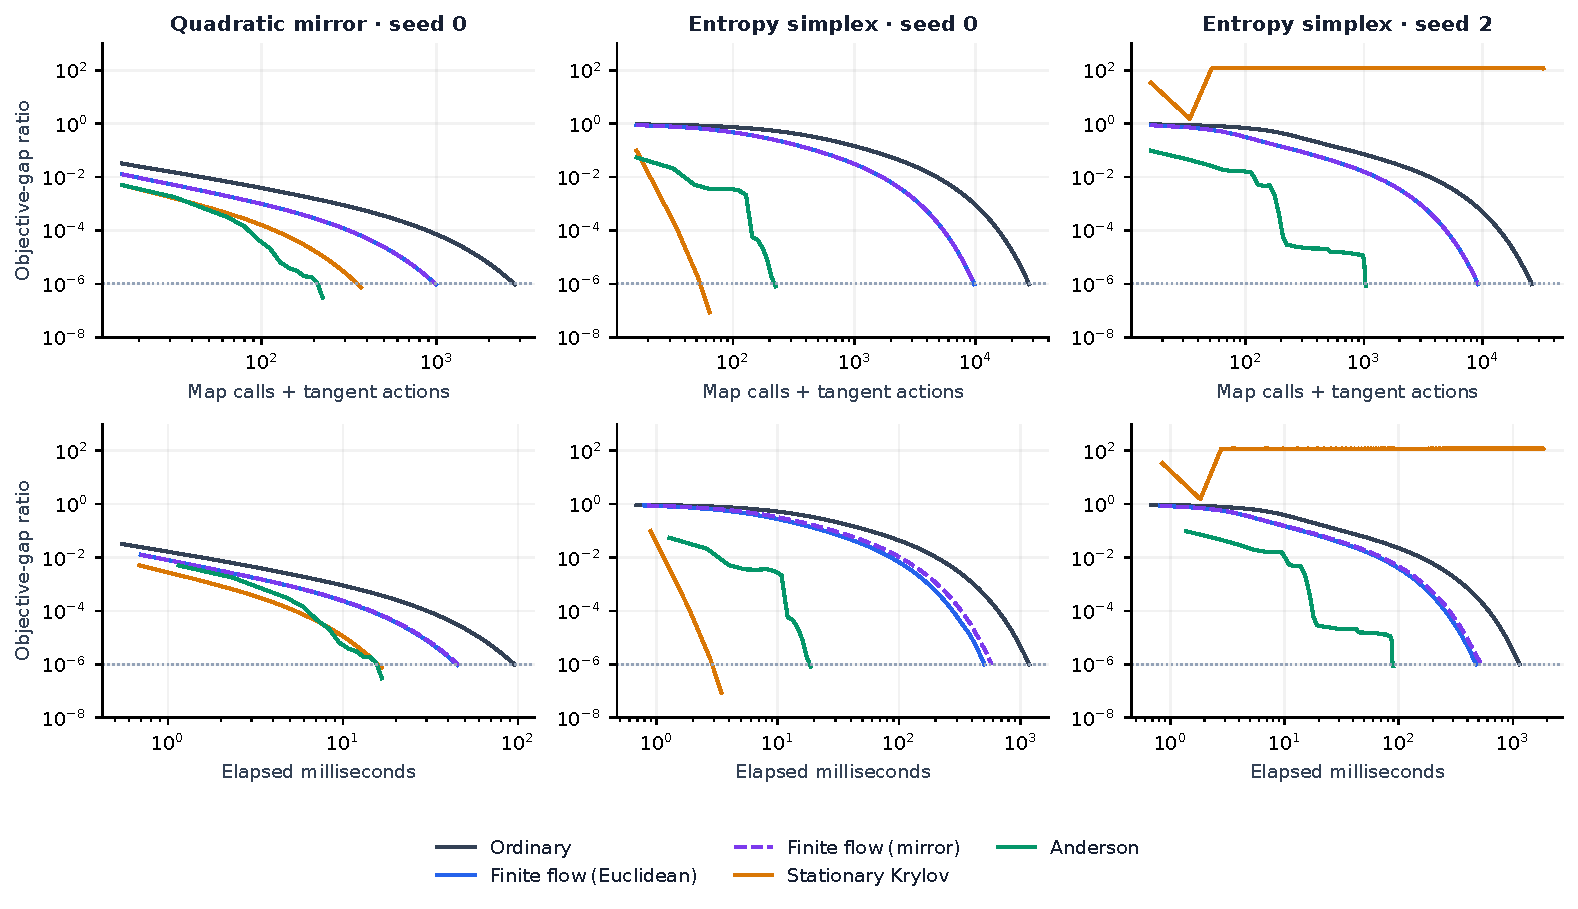
\includegraphics[width=\textwidth]{figures/pilot_curves.pdf}

\caption{Representative primary traces at $n=512$. The top row counts maps and tangent actions; the bottom row uses elapsed time from the first timed repeat. Euclidean and mirror finite-flow work curves nearly coincide. Entropy seed two exposes the stationary comparator\textquotesingle s failure. Tables use all seeds and repeated timing medians.}

\label{fig:curves}\end{figure}

\subsection{Penalty sensitivity and the shadow-coordinate result}

The penalty screen keeps the acceleration schedule fixed. For $\rho=1$, both finite and stationary Krylov schedules fail on all three seeds while ordinary ADMM and Anderson reach the target. At $\rho=10$, finite flow succeeds on only one seed. The exact shadow reparameterization preserves ordinary ADMM numerically and reduces state dimension, but does not resolve these failures. Thus an off-graph extrapolated memory state is not a sufficient explanation: the frozen geometric prediction itself remains inadequate.

\begin{table}[htbp]\centering\small

\begin{tabular}{r rrrrr}\toprule

$\rho$ & Finite, full & Finite, shadow & Stationary, full & Stationary, shadow & AA, shadow\\\midrule

0.001 & 1.52 & 1.70 & 4.19 & 5.63 & 2.44\\

0.01 & 1.28 & 1.41 & 1.65 & 1.45 & 0.92\\

0.1 & 0.55 & 0.61 & 0.57 & 0.62 & 0.64\\

1 & -- (0/3) & -- (0/3) & -- (0/3) & -- (0/3) & 1.23\\

10 & -- (1/3) & -- (1/3) & -- (0/3) & -- (0/3) & 1.85\\

\bottomrule\end{tabular}

\caption{Median elapsed-time speedup relative to ordinary iteration in the same representation, at $n=256$. Values above one are faster. Any unsuccessful seed replaces the ratio by its success count. The full and shadow representations have the same ordinary trajectory and target.}

\label{tab:penalty}\end{table}

\begin{figure}[htbp]\centering

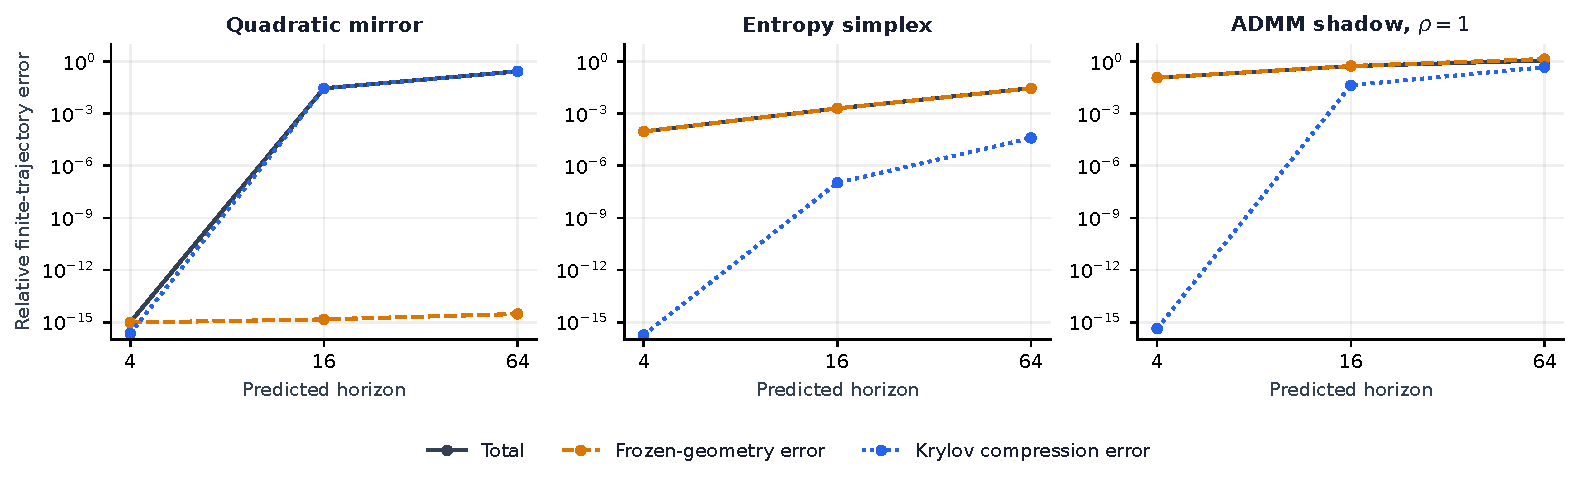
\includegraphics[width=\textwidth]{figures/error_sources.pdf}

\caption{Independent one-block diagnostics at ordinary prefix four, Krylov depth four, seed zero. Errors are normalized by the actual finite displacement; curves at $10^{-16}$ represent the plotting floor. The affine quadratic primarily exposes compression error. Nonlinear and active-mask geometry can dominate in the other examples. All reference map calls and full tangent recurrences used for this figure are separately charged diagnostics, excluded from accelerated solve timings.}

\label{fig:defects}\end{figure}

The boundary-drift control has an exact rank-one finite flow and a singular stationary projected system. Its horizon-sixteen Python implementation still does not beat the extremely cheap ordinary update in elapsed time. This makes the distinction between an exact transport representation and a practical acceleration particularly clear.
